\documentclass[a4paper, 11pt]{article}

% Nécessaire
\usepackage[utf8]{inputenc}
\usepackage[T1]{fontenc}
\usepackage{lmodern}

% Biblio
\usepackage{natbib}
\bibliographystyle{abbrvnat}
\usepackage{hypernat}
\bibpunct{\textcolor{blue}{[}}{\textcolor{blue}{]}}{}{a}{\textcolor{blue}{,}}{;}

\usepackage[french]{babel}
\usepackage{amsmath, amsthm}
\usepackage{amsfonts,amssymb}

% Marge
\usepackage{geometry}
\geometry{margin={2.2cm ,2cm}}

% Figures, graphiques
\usepackage{graphicx}
\usepackage{epsfig}
\usepackage{caption}

% Surlignage
\usepackage{alltt}

\usepackage{xcolor}
\usepackage{soul}
\usepackage{color}
\usepackage{colortbl}

% Indicatrice
\usepackage{dsfont}

\usepackage{multirow}
\usepackage{eurosym}
\usepackage{extarrows}
\usepackage[colorlinks=true, citecolor=blue, linkcolor=.]{hyperref}

% Graphique
\usepackage{tikz}


% Titre
\title{Exploration de l'aspect disponibilité en ressources du modèle}
\author{}
\date{}



\begin{document}
 \maketitle
 
 La disponibilité en ressources de notre modèle est depuis le début définit par
 \[
  R = \max\left\{1, k\frac{I}{N}\right\}.
 \]
 Pour l'instant, ce coefficient ne donne pas l'impression d'avoir un impact notable sur le modèle.
 
 L'idée est d'alors de remplacer $R$ par un coefficient $k(t)$ libre chaque jour et pour chaque sous-bloc, de sorte que le modèle puisse ajuster aux mieux nos données sur nos observations. Et ensuite essayer de déterminer s'il y a une relation entre $k(t)$ et $I/N$ ou $N/I$.

 Comme prévu, le modèle arrive à bien ajuster aux données observées comme le montre la figure~\ref{toto}.
 \begin{figure}[ht]
  \centering
  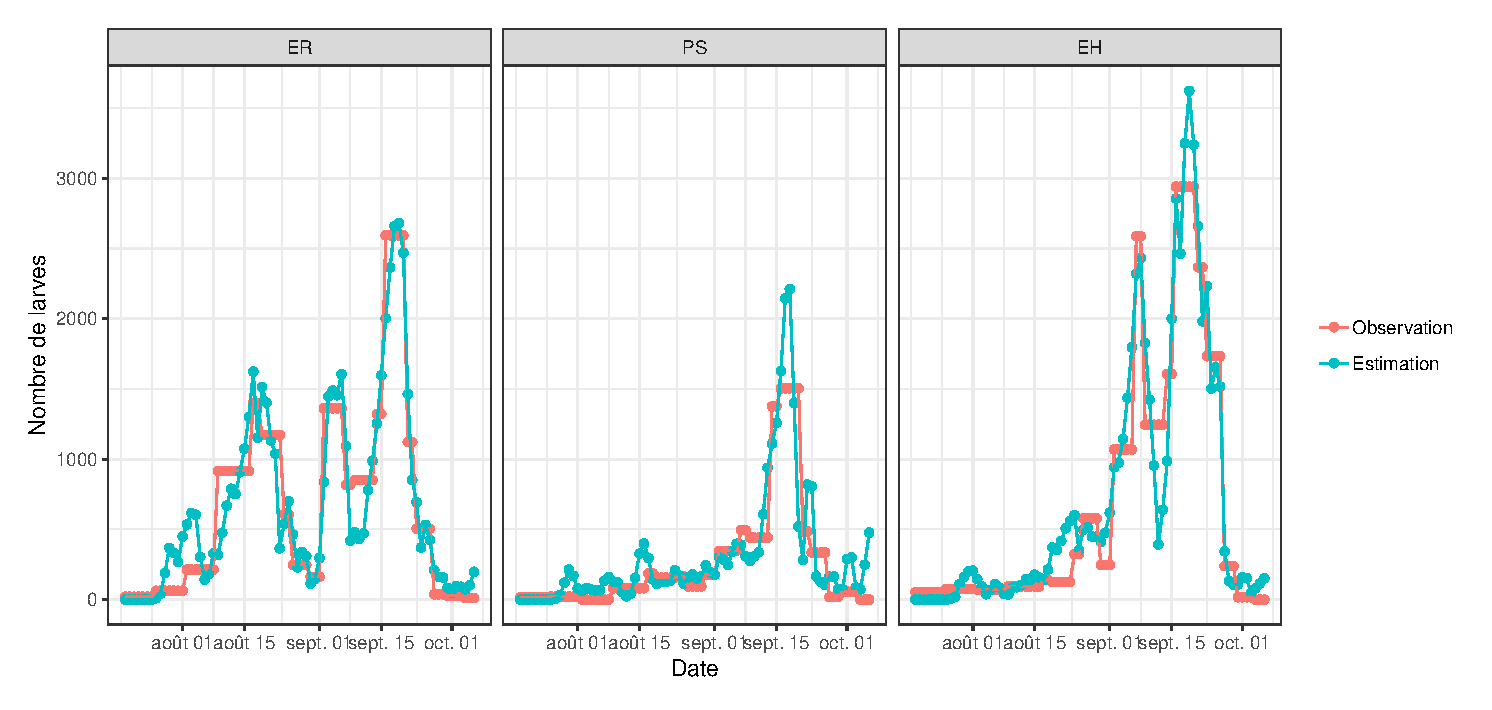
\epsfig{file = plots/ressource_libre.eps, scale = 0.65}
  \caption{Résultats de la calibration avec un paramètre libre $k(t)$ chaque jour pour chaque sous-bloc.}
  \label{toto}
 \end{figure}

 Malheureseument, comme le montre les figures \ref{tutu} et \ref{titi}, il ne semble pas y avoir de lien entre $k(t)$ et les ratio précedemment mentionnés.
 
 
  \begin{figure}[ht]
  \centering
  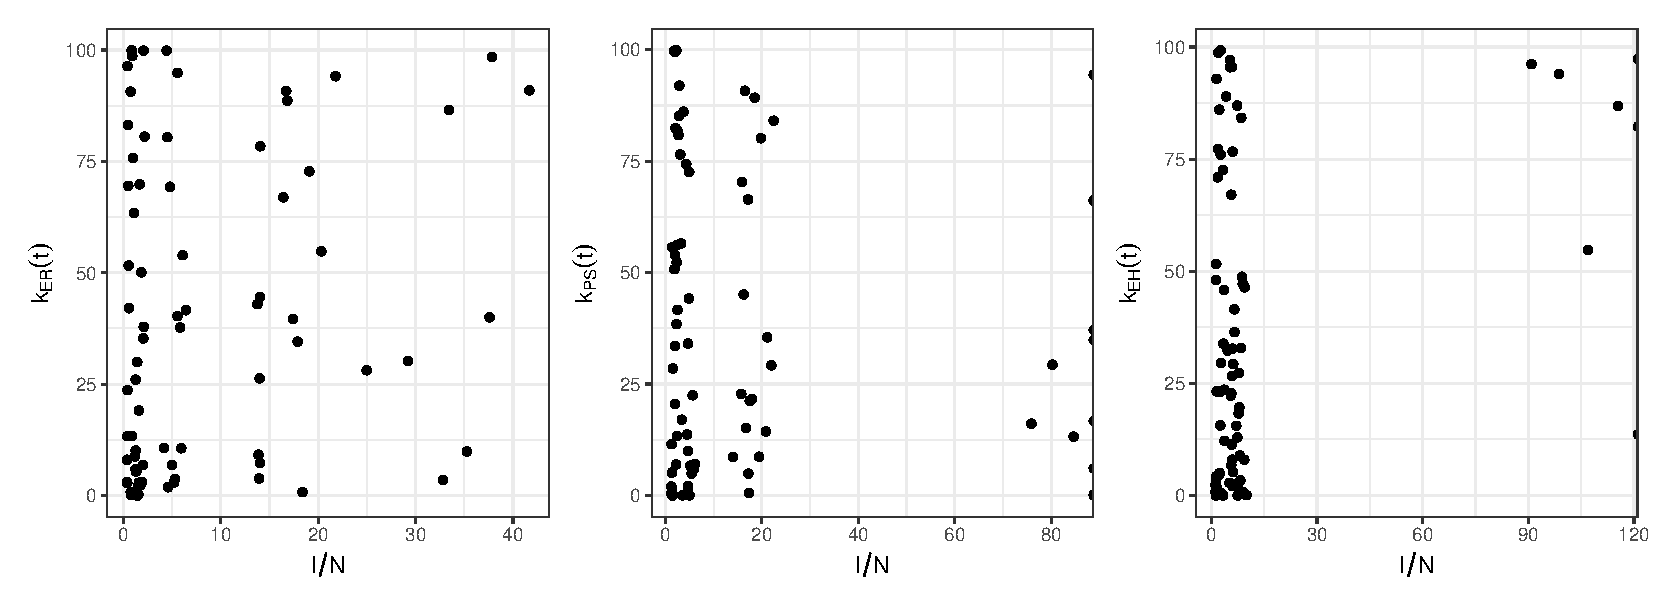
\epsfig{file = plots/kisurn.eps, scale = 0.60}
  \caption{$k(t)$ en fonction du ratio $I/N$.}
  \label{tutu}
 \end{figure}

  \begin{figure}[ht]
  \centering
  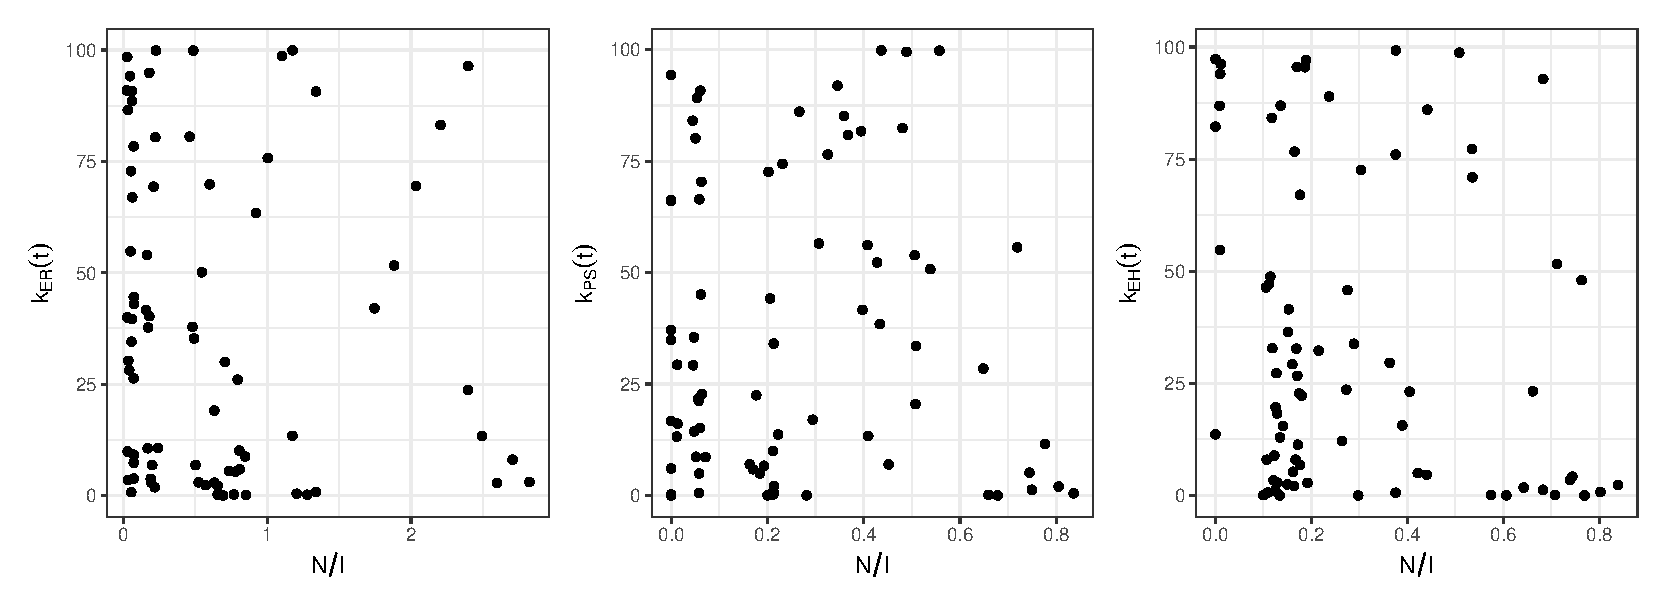
\epsfig{file = plots/knsuri.eps, scale = 0.60}
  \caption{$k(t)$ en fonction du ratio $N/I$.}
  \label{titi}
 \end{figure}

 
 
\end{document}
